\section{Problem formulation}





%\\Visualizing a large collection of trajectories are used frequently in map service or smart city applications.
When exploring a large collection of trajectories, efficient and effective large-scale trajectory visualization is challenging in both academia and industry.
The reasons are (i) the size of trajectory data is very large (e.g., several GB in an hour),
and (ii) the limited rendering ability of existing commercial graphics device (e.g., XXX).

Sampling is a delta-facto solution for the problems with big data. 
Many exiting visual analytics systems leverage powerful database manage system as the backend to facilitate the fast data processing. Based on the solution proposed in ScalaR~\cite{battle2013dynamic}, a common visualization framework involving sampling technique is illustrated as Figure~\ref{fig:framework}, where a sampling layer is set between the backend and frontend. Since the sampling methods are always designed for complicated task, the algorithms may not be efficient enough to support the interactive data exploration. Thus the cache model is always implemented to save the sampling results. In our scenario, the users query large amount of data(e.g. all Shenzhen trajectories in one week) once and then conduct interactive multi-resolution exploration based on the sampled data, thus the method need to guarantee the visual quality well across different resolutions.

Target at the sampling requirement, the naive solutions such as uniform random sampling cannot generate acceptable because the serious visual information loss. In this section, we first define a loss function to evaluate the visual quality between the visualization results between whole dataset and sampled subset. Then we analyze the hardness of the problem and design algorithms for it.  
%A naive solution to employ sampling idea for large-scale trajectory visualization problem is randomly selecting several trajectories from the data set then visualize it by graphics device.
%However, the visualization result may be not acceptable by the user.
%In this work, we study the large-scale trajectory visualization problem.
%In particular, we focus on visual quality guaranteed sampling method for large trajectory data visualization.
%The major challenges to design visual quality guaranteed sampling method are:
%(I) how to define visual quality theoretically? (II) how to guarantee the quality of the sampling-based visualization result?
%In this work, we first formate visual quality by defining the loss function between the visualization results of the whole dataset and sampled dataset.
%\\With the loss function, we analyze the hardness of the problem, and devise a visual quality guaranteed sampling algorithm for it.



\begin{figure}[t]
	\centering
	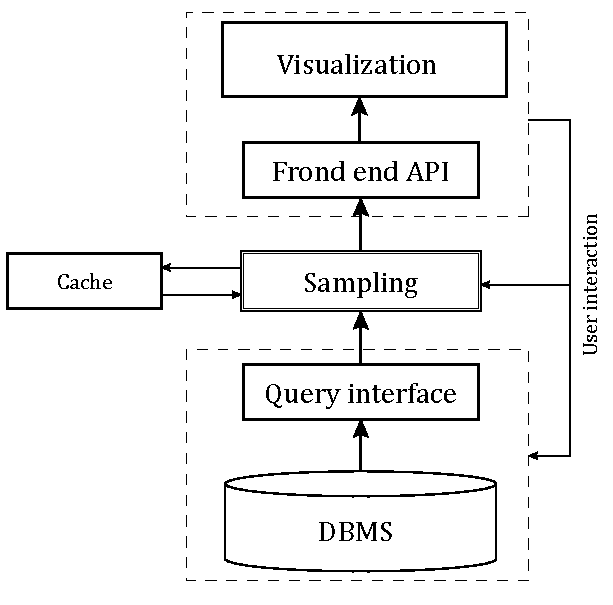
\includegraphics[width=0.3\textwidth]{pictures/framework/DBVAframework.pdf}
	\vspace{-5mm}
	\caption{A visualization framework involving sampling layer between the front-end and database management system.}
	\vspace{-5mm}
	\label{fig:framework}
\end{figure}



\subsection{Problem description}
\begin{problem}[Sampling-based trajectory visualization problem]\label{prob:def}
Given a large-scale trajectory dataset $\D$ and an integer $k$,
the trajectory visualization problem is selecting a subset of trajectories $\oR \subseteq \D$, such that loss function $loss(\oR,\D)$ is minimized.
\end{problem}

From the user’s perspective, there are many ways to define the loss function $loss$ between the visualization result qualities of the sampled subset $\oR$ and the whole dataset $\D$.
For example, \cite{park2016visualization} defined point-based loss function for very large scatter points visualization.
However, it is not applicable for trajectory data visualization.
In order to address that, we propose an novel loss function for trajectory visualization problem.

Intuitively, the visual quality difference between the visualization results of two trajectory datasets depends on the user specified visualization level of details (a.k.a., LOD).
Given an empty canvas (e.g., displaying device) with a user specified level of details, 
the visualization process is rendering the trajectories into canvas with the given level of details (e.g., the number of pixels in each row and each column).
Considering a trajectory data set $\D$ and a subset of trajectories $\oR \subseteq \D$,
The visual quality loss between $\oR$ and $\D$ is defining as the different pixels of the visualization results about $\oR$ and $\D$ in the canvas with specified LOD.
We then define the loss function of sampling-based trajectory visualization problem as $loss(\D, \oR) = \frac{\V(\D) - \V(\oR)}{\V(\D)}$,
where $\V()$ measures the number of rendered pixels in the canvas of a given trajectory dataset.

Given a trajectory data set $\D$ and an integer $k$,  our research objective is finding subset $\oR$, such that  the visualization quality loss function $loss(\D, \oR)$ is minimized,
i.e.,
$$ \min_{\oR \subseteq \D, |\oR| = k}  loss(\D, \oR) =  \frac{\V(\D) - \V(\oR)}{\V(\D)}. $$ %\\ %\nonumber


%  \Leftrightarrow  & \min_{\oR \subseteq \D, |\oR| = k}  \V(\D) - \V(\oR) \\ \nonumber
%  \Leftrightarrow  & \min_{\oR \subseteq \D, |\oR| = k}  \sum_{\forall \D_i \in \D} \V(\D_i) - \V(\oR)
%Intuitively, the visualization quality from user's perspective highly depends on the resolution of displaying device,
%e.g., the number of distinct pixels in each dimension that can be displayed.

%Given a high resolution displaying device, data objects set $\D$, and a subset of data objects $\oR \subseteq \D$.
%The visualization quality loss between $\oR$ and $\D$ is defining as the different pixels of the visualization results of $\oR$ and $\D$ in the given display device.
%Given a trajectory data set $\D$ and an integer $k$,  our research objective is selecting a sized-$k$ subset of trajectories which minimize
%the visualization quality loss function $loss(\D, \oR)$.
%Formally, the loss function is defined as $loss(\D, \oR) = \V(\D) - \V(\oR)$.



\subsection{Hardness analysis}
In real-world applications, the pixels in canvas will be rendered by different colors according to the specified visualization scheme.
For the sake of presentation, we analyze the hardness of our research objective with a simple render manner of visualization result.
In particular, for each pixel in the canvas, it will be rendered if there is a trajectory pass through it, otherwise it will not be rendered.
Suppose each pixel in the canvas has an unique id, let $\U$ be the universal set of all pixels in the canvas
For each trajectory $\D_i \in \D$, it consists of a set of pixels in the canvas, e.g., it is a subset of $\U$.
Thus, the subset $\oR$ also is a subset of $\U$ as $\oR = \cup_{\oR_i \in \oR} \oR_i$.

Our research objective is minimizing loss function $loss(\D, \oR) =  \frac{\V(\D) - \V(\oR)}{\V(\D)}$.
Obviously, the visualization result of $\D$ is a constant value, denotes as $\mathsf{C}$.
Our research objective of Problem~\ref{prob:def} can be transformed as follows:
\begin{align}\label{eqn:obj2} \nonumber
\text{Objective}: & \min_{\oR \subseteq \D, |\oR| = k}  \frac{\V(\D) - \V(\oR)}{\V(\D)} \\ \nonumber
& \Leftrightarrow \min_{\oR \subseteq \D, |\oR| = k}  \frac{\mathsf{C} - \V(\oR)}{\mathsf{C}} \\ \nonumber
& \Leftrightarrow \max_{\oR \subseteq \D, |\oR| = k}  \cup_{\oR_i \in \oR} \oR_i
\end{align}

It is equivalent to select sized-$k$ trajectory set $\oR$ from $\D$ which $\cup_{\oR_i \in \oR} \oR_i$ is maximized.

It is a typical set cover maximization problem\footnote{\url{https://en.wikipedia.org/wiki/Maximum_coverage_problem}}, which is a well-known NP-hard problem in literature.

%It is equivalent to select sized-$k$ trajectory set $\oR$ from $\D$ which $\cup_{\oR_i \in \oR} \oR_i$ is maximized.
%It is a NP-hard problem as we proved in Lemma~\ref{lem:np}.

%\begin{lemma}[NP hard]~\label{lem:np}
%Given a trajectory dataset $\D$ and an integer $k$, 
%The sampling-based trajectory visualization problem (see Problem~\ref{prob:def}) is NP-hard.
%\end{lemma}

%We omit the proof of Lemma~\ref{lem:np} as it is a typical set cover maximization problem\footnote{\url{https://en.wikipedia.org/wiki/Maximum_coverage_problem}}, which is a well-known NP-hard problem in literature.

